\chapter{Optimized high-dimensional representation in spiking neurons}
The implementation of a Semantic Pointer Architecture in a spiking neural network requires the representation of high-dimensional vectors with a certain accuracy.
One of the main factors influencing the accuracy is the number of neurons.
A higher number of neurons improves accuracy and, unfortunately, increases simulation times.
If the accuracy of the representation can be improved in a different way, it would allow to reduce the neuron number accordingly and reduce simulation times without sacrificing accuracy.
I previously proposed one such optimization method \parencite{gosmann216}, which improved the accuracy of SPA operations by up to 25 times.
Here, I will describe a more general applicable method that supersedes the previous method by matching or exceeding the previously achieved performance.
The new method also has a number of additional advantages.
It does not require any prior simulation to obtain empirical noise estimates and is simpler in its implementation.

\section{Types of error in neural representations}
In the NEF the total mean representational error is given by
\begin{equation}
    \errtotal^2 = \left\langle \errtotal^2(\vc x) \right\rangle_{\!\vc x \in \repspace} = \left\langle \norm{\vc x - \hat{\vc x}(t)}^2 \right\rangle_{\!t,\,\vc x \in \repspace} \text{.}
\end{equation}
As detailed by \textcite[47--48]{eliasmith2003} the total error is constituted out of the error caused by spiking noise $\errnoise$ and the error due to the static distortion $\errdist$ from the imperfect decoding:
\begin{align}
    \errtotal^2(\vc x) &= \errnoise^2(\vc x) + \errdist^2(\vc x) \\
    \errnoise(\vc x) &= \left\langle \norm{\hat{\vc x}(t) - \langle \hat{\vc x}(t) \rangle_{\!t}}^2 \right\rangle_{\!t} \\
    \errdist(\vc x) &= \norm{\vc x - \langle \hat{\vc x}(t) \rangle_{\!t}}^2 \text{.}
\end{align}
The relation of the error terms is explained by the partitioning of the sum of squares in ordinary least squares model (which is used to solve for decoders in the NEF).
Note that the noise error will depend on the decoding synapse.
As $\syntau \rightarrow \infty$, the noise error will approach zero ($\errnoise \rightarrow 0$).
Because the synapse limits how fast the neural representation can be updated, we get a trade-off of the noise in the system and how fast it reacts to new inputs.

Due to the neuron nonlinearities, finding analytical solutions for the error terms is likely not possible (except for constrained special cases).
However, we can estimate the error terms from computational experiments.
To do so, we sample $\vc x \in \repspace$ or use a regular grid of $\vc x$.
Each $\vc x$ is then presented for some duration $\Delta t_{\ped{ss}}$ to reach the steady state and then $\hat{\vc x}(t)$ is measured for some sample duration $\Delta t_{\ped{sample}}$.
Appropriate durations will depend on the decoding synapse (longer synapses require more time to reach the steady state) and firing rate (a longer sampling duration is required for accurate estimates with low firing rates).

As the dimensionality of the higher-dimensional space increases, it becomes increasingly difficult to cover the whole space with samples from $\repspace$.
Most of the time, though, we can treat the space as an isotropic hyperball, i.e.\ it does not matter along which direction we move through the space.
This requires that the NEF ensemble's encoders are uniformly sampled from the hypersphere surface which is usually the case (but there are some exceptions like certain implementations of a product network,~\cite{gosmann2015-1}, or thresholding ensembles, \cref{sec:thresholding}).
Without loss of generality, we assume the representational radius of the hyperball to be $r = 1$ (as it is purely a scaling factor).
The isotropy property allows us to cut through the center of the hyperball with a one-dimensional line.
Measuring the error $\err(x) = \err(\vc x)$ at $m$ regular spaced points $\vc x_i = (x_i, 0, \dotsc, 0)\Tr$ with $x_i = i * \Delta x - \Delta x/2,\ \Delta x = 1/m,\ 1 \leq i \leq m$ along such a line, the mean error for the hyperball can be estimated as
\begin{align}
    \err &= \frac{\sa_{\dims}}{\ballvol} \sum_{i=1}^{m} \err(x_i) \cdot \Delta x \cdot r(x_i) \\
    \sa_{\dims} &= \frac{2 \pi^{\dims/2}}{\gammafn(\dims/2)} \\
    \ballvol &= \frac{\pi^{\dims/2}}{\gammafn\!\del{\frac{\dims}{2} + 1}} \\
    r(x) &= \frac{1}{q} \sum_{i=1}^{q} \abs{x - \del{1 + \frac{1}{q}} \frac{\Delta x}{2} + i \frac{\Delta x}{q}}^{\dims - 1}
\end{align}
where $\sa_{\dims}$ is the $\dims$-dimensional solid angle, $\ballvol$ the volume of a $\dims$-ball with radius $\radius = 1$, and $r(x)$ estimates the radius to the power of $\dims-1$ for an $x$ with $q$ evaluation points.
This later estimation of the radius across the $\Delta x$ interval is necessary to not under- or overestimate the integral by a large amount.
This were to happen if only the radius at the exact evaluation point would be used.


\section{Properties of the error in neural representations}
When looking at the representation of a spiking neural network, the noise error is the main factor to consider.
It will go down by $\bO(1/\sqrt{n})$ where $n$ is the number of neurons (\cref{fig:noise-error}a), whereas the distortion error will decrease by $\bO(1/n)$.
The total error is thus dominated by the noise error for a sufficient number of neurons \parencite[Fig.~2.6]{eliasmith2003}.
In contrast, for rate neurons without spiking noise ($\errnoise = 0$) and only the distortion error is relevant.
Furthermore, with the Nengo default parameters the noise error in the NEF the increase in the noise error with dimensions $\dims$ will be in $\bO(d)$ (\cref{fig:noise-error}b).
\begin{figure}
    \centering
    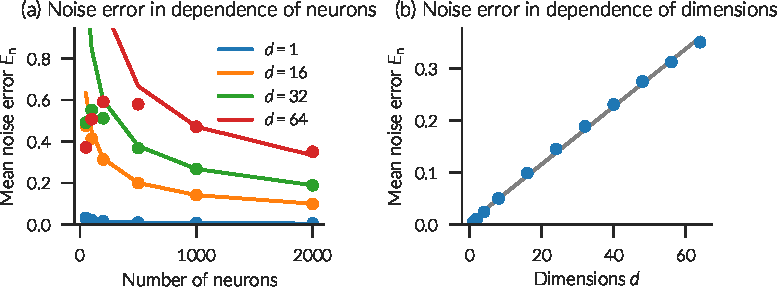
\includegraphics{figures/noise-error}
    \caption[Mean noise error with $\csdist(\dims + 2)$ distributed intercepts]{The mean noise error $\errnoise$ in dependence of (a) the number of neurons and (b) the number of dimensions. Scatter points show empirically determined values with \SI{95}{\percent} confidence intervals smaller the marker size. Solid lines in (a) are extrapolated from the mean values for \num{1000} neurons assuming the noise error is in $\bO(n)$. The solid gray line in (b) is a linear regression through all shown data points.}\label{fig:noise-error}
\end{figure}

When looking at the error along a line through the hyperball (\cref{fig:error-linecut}), it becomes apparent that the distortion is mostly flat, but increases near the surface.
The noise error will be slightly larger in the center of the ball than towards the surface with higher dimensionalities (it is a flat line for $\dims = 1$).
Both of these effects become more pronounced as the dimensionality increases.
Moreover, the one-dimensional cut shows a distorted picture of the importance of different regions in the distortion.
As the dimensionality increases, the most of the volume of the hyperball will be close to the surface.
Thus, the distortion (and noise) close to $-1$ and $1$ of the cut will come to dominate the mean error.

The main cause for the observed shape of the distortion is the uniform sampling of evaluation points from the hyperball (\cref{fig:circle-covering}).
When looking at the convex hull of the sample points, this hull will always be smaller than the hyperball (even if some evaluation points are exactly on the surface).
Thus, parts of the hyperball near the surface are not covered by the evaluation points and will not be considered in the least squares optimization of the decoders.
As the number of dimensions increases, this will become a bigger problem as the volume for a hyperball goes to zero as $\dims \rightarrow \infty$ (all of the ball will be surface).
To show that this distortion is indeed caused by the partial covering, we can increase the radius of the hyperball for sampling the evaluation points slightly to cover more of the unit-ball.
This is done in \cref{fig:error-radius-scale} for a 64-dimensional representation with \num{50}~neurons per dimension (\num{3200} in total).
While this makes the distortion more even (mean distortion reduced by \num{0.011}), it unfortunately also increases noise level (by \num{0.019}) because evaluation points have a larger spacing now.\footnote{Both values are statistically highly significant with $p \approx 0$ as determined by bootstrapping.}
\begin{figure}
    \centering
    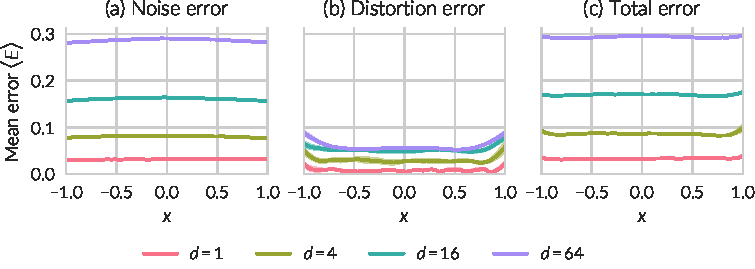
\includegraphics{figures/error-linecut}
    \caption[Mean error along line cut through hyperball]{Mean error along a line cut through the $d$-dimensional hyperball with $50\dims$ neurons. The (a) noise error component, (b) distortion error component, and (c) the total error are shown. The shaded regions indicate \SI{95}{\percent} confidence intervals.}\label{fig:error-linecut}
\end{figure}
\begin{figure}
    \begin{captionbeside}[Covering of the unit-circle with evaluation points]{Covering of the two-dimensional unit-circle with 50~uniformly sampled evaluation points. The orange, shaded region shows the convex hull which fails to cover the area close to the circle boundary.}[i]
        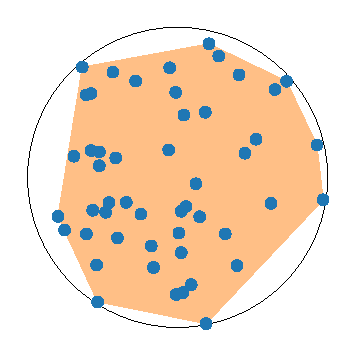
\includegraphics{figures/circle-covering}
    \end{captionbeside}\label{fig:circle-covering}
\end{figure}
\begin{figure}
    \centering
    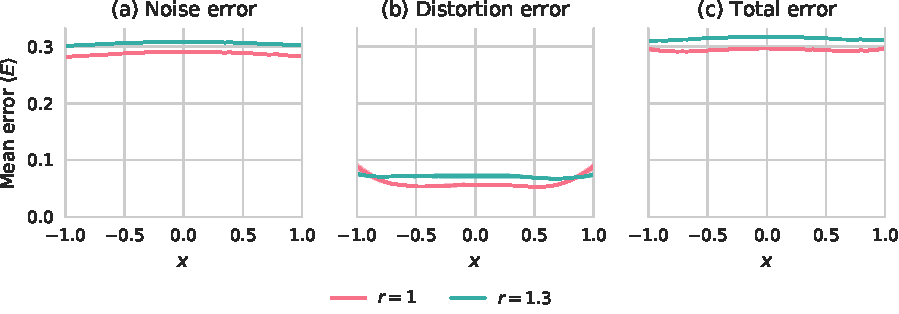
\includegraphics{figures/error-radius-scale}
    \caption[Mean error along line cut through hyperball with scaled evaluation point radius]{Mean error along a line cut through the \num{64}-dimensional hyperball with \num{3200} neurons and different radii $r$ from which evaluation points are picked. The shaded regions indicate \SI{95}{\percent} confidence intervals.}\label{fig:error-radius-scale}
\end{figure}

Vectors in the SPA are often of unit-length and thus a good, low-distortion representation of the hyperball surface is desirable.
Unfortunately, I am not aware of any method to flatten out the distortion at the surface without a higher increase in noise error.
To completely cover the ball in a convex hull of evaluation points, it is necessary to place some evaluation points outside of the ball which will cover and optimize for space outside of the representational space.
This will lead to a trade-off of flatness of the distortion and baseline of the distortion.
Ultimately, the problem of distortion is minor as for spiking neurons the error is dominated by the noise component.


\section{Effect of the intercept distribution on noise and distortion}
The intercepts in Nengo are chosen to be distributed uniformly by default.
In higher dimensions, this has the effect that most neurons are either almost never or almost always active for values in the representational space (\cref{fig:act-proportion}).
Neurons that are always silent do not contribute to the representation as they provide no information about the represented value.
But also always active neurons only contribute minimally to the representation.
Even though the firing rate will still vary a bit over the representational space, the response curve is steepest and carries the most information closest to the intercept for most neuron models.
The mapping of a small change in the represented value to a large change in firing rate also allows for a less noisy decoding as a single spike will change the decoded value less.
\begin{figure}
    \centering
    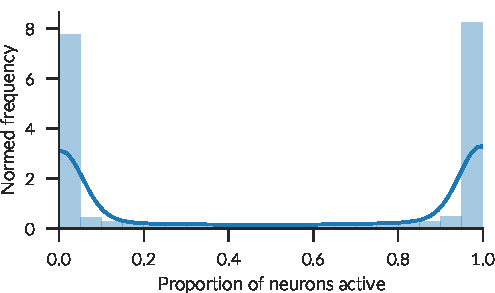
\includegraphics{figures/act-proportion}
    \caption[Distribution of the proportion of active neurons]{Histogram (shaded bar plot) and kernel-density estimate (line) of the proportion of neurons active for uniformly sampled 64-dimensional vectors.}\label{fig:act-proportion}
\end{figure}

Thus, a better intercept distribution should have less neurons that are barely ever active, but should also distribute the intercepts so that there is an even distribution of the fraction of space a neuron is active for.
The latter criterion can be achieved by distributing the intercepts according to $\csdist(\dims+2)$ where $\csdist(d_{\csdist})$ is the distribution of cosine similarities between random uniformly distributed $d_{\csdist}$-dimensional unit-vectors.
Its probability density function is given by (also see \cref{fig:cosine-sim}, derivation in \cref{apdx:cosine-sim})
\begin{equation}
\pcs(x; d_{\csdist}) = \frac{1}{B\!\del{\frac{1}{2}, \frac{d_{\csdist} - 1}{2}}} \cdot \del{1 - x^2}^{\del{d_{\csdist} - 3} / 2},\quad x \in [-1, 1] \text{.}\label{eqn:pcs}
\end{equation}
$\csdist(\dims+2)$ is equivalent to the distribution of single coordinates of points uniformly sampled from within the $\dims$-dimensional unit-ball \parencite{voelker2017}.
Thus, by using this intercept distribution, the frequency of intercepts corresponds to the distribution of $\langle \vc x, \enc \rangle,\ \vc x \in \repspace$, i.e.\ values in the representational space projected onto the (uniformly distributed) neuron encoders.
Note that for $\dims = 1$, $\csdist(\dims + 2)$ will be the uniform distribution.
\Cref{fig:act-cs} compares the relative amount of neurons that do not fire for any of the evaluation points.
For the standard uniform distribution, this fraction rises to above \num{0.35}, but is close to zero with the cosine similarity intercept distribution.
\begin{figure}
    \centering
    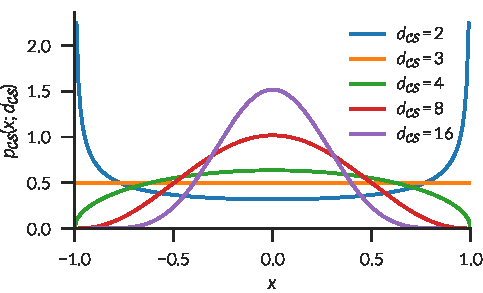
\includegraphics{figures/cosine-sim}
    \caption{PDF $\pcs(x; d_{\csdist})$ of the cosine similarity distribution}\label{fig:cosine-sim}
\end{figure}
\begin{figure}
    \centering
    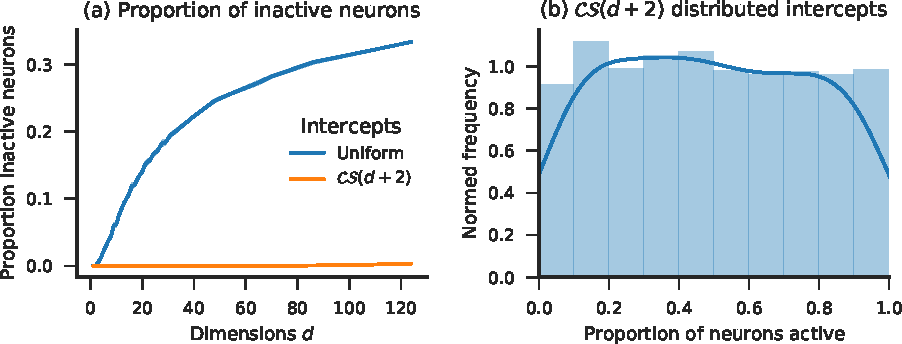
\includegraphics{figures/act-cs}
    \caption[Proportion of inactive neurons and its distribution]{(a) Proportion of neurons inactive for all \num{10000} uniformly sampled $\dims$-dimensional vectors. The proportion is plotted for neural ensembles with a uniform intercept distribution (blue) and intercepts distributed according to $\csdist(\dims + 2)$ (orange). The shaded areas denote \SI{95}{\percent} confidence intervals. (b) Histogram (shaded bar plot) and kernel-density estimate (line) of the proportion of neurons active for uniformly sampled 64-dimensional vectors when distributing intercepts according to $\csdist(\dims + 2)$.}\label{fig:act-cs}
\end{figure}

While this gives a mathematical motivation to choose this intercept distribution, it must be shown empirically that it performs better than a uniform intercept distribution.
In the following I will present a number of experiments to make this case and give an intuition about the effect of this particular intercept distribution.
Further evidence is presented in \cref{apdx:hdrep}.
All experiments have been performed with $\dims = 64$ dimensional representations and $50 \dims = 3200$ spiking LIF neurons as long as not otherwise noted.
For each experiment 15 samples using different random number seeds were obtained.
The benefit of choosing the $\csdist(\dims + 2)$ intercept distribution will be larger for increasing dimensionality, but 64 dimensions is sufficient to see a clear effect.
For fewer dimension the benefit will be less, but not worse than the uniform intercept distribution (\cref{apdx:hdrep}).
This is consistent with the $\csdist(\dims + 2)$ distribution approaching a uniform distribution for $\dims \rightarrow 1$.
The asymptotic scaling of the noise error component with the number of neurons does not change for the given choices of the intercept distribution.
In so far any neuron number that is large enough for the noise error to dominate can be used in these experiments and noise error values for other neuron numbers can be extrapolated.
This might invalidate the results for small neuron numbers, but such cases should be considered as special with any intercept distribution.
Finally, spiking LIF neurons are of primary interest as most commonly used neuron model in the NEF\@.
But I will give some consideration to other neuron types in \cref{apdx:hdrep}.
Any stated differences in error will be based on the aforementioned parameters.
Furthermore, all stated differences have been found to be statistically highly significant with $p \approx 0$ using bootstrapping.

The basic effects of the $\csdist(\dims + 2)$ intercept distribution can be seen in \cref{fig:error-cs-intercepts}.
The total mean error is reduced by \num{-0.130}.
This is mainly due to a reduction in the noise error.
The distortion seemingly increases, but because most of the volume of the space is near the surface and the distortion there ends up a little bit lower, the total mean distortion will also decrease (\num{-0.020}).
However, where the space is distorted changes.
While the uniform distribution leads to an even distortion except towards the hypersphere surface, the cosine similarity distribution gives a distortion that varies more across the space.
In particular, there is a ring of higher distortion between the center and the surface of the hyperball and another such ring around the surface.
\begin{figure}
    \centering
    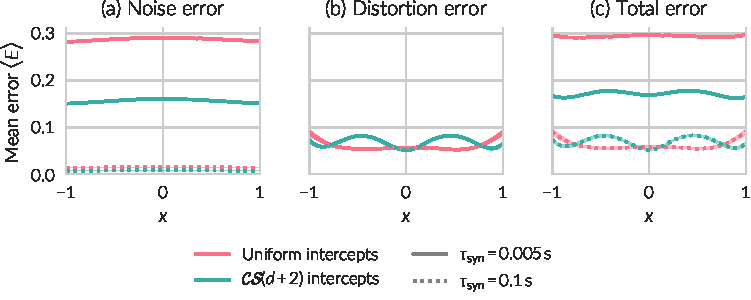
\includegraphics{figures/error-cs-intercepts}
    \caption[Mean error along line cut with different intercept distributions]{Mean error along a line cut through the 64-dimensional hyperball with \num{3200}~neurons, different intercept distributions (pink vs.\ turquoise) and different synaptic time constants (solid vs.\ dotted line). The shaded regions indicate \SI{95}{\percent} confidence intervals.}\label{fig:error-cs-intercepts}
\end{figure}

In general, there will be a noise-distortion trade-off.
Reducing the noise error by changing the intercept distribution, will lead to a more uneven distortion and can potentially increase the total distortion.
For spiking neurons with short synaptic time constants, the noise error is usually much higher and thus the change in the distortion will often be negligible.
Longer synaptic time constants will shift this trade-off as the noise error will be lower.
Still, for biological realistic time constants of up to \SI{0.1}{\second}, the cosine similarity intercept distribution will perform better.
It is also worth noting that this trade-off will be slightly affected by the regularization term when solving for the decoders (\cref{fig:error-cs-intercepts-reg}).
A higher regularization will decrease the noise as the decoders get less sensitive to small fluctuations, but increases the distortion towards the hypersphere surface.
The opposite effects are observed with less regularization.
\begin{figure}
    \centering
    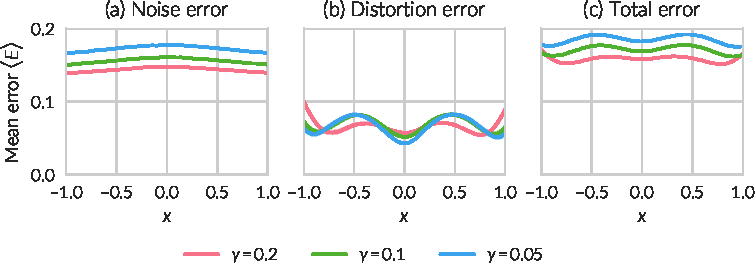
\includegraphics{figures/error-cs-intercepts-reg}
    \caption[Mean error along line cut with different regularization]{Mean error along a line cut through the 64-dimensional hyperball with \num{3200}~neurons and different regularization $\reg$. The shaded regions indicate \SI{95}{\percent} confidence intervals.}\label{fig:error-cs-intercepts-reg}
\end{figure}

Interestingly, the cosine intercept distribution does not only reduce the noise by a constant factor compared to the uniform distribution.
Rather it improves the scaling of the noise error from $\bO(d/\sqrt{n})$ to $\bO(d^{3/4}/\sqrt{n})$ (\cref{fig:cs-error-scaling}).
\begin{figure}
    \centering
    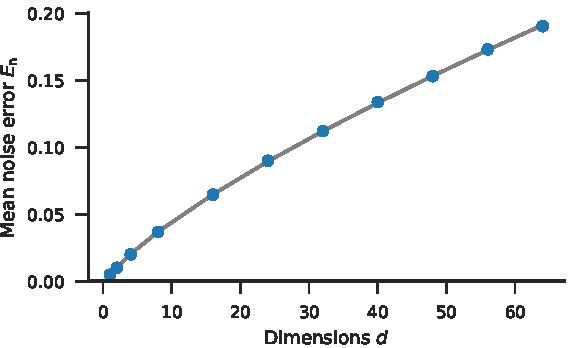
\includegraphics{figures/cs-error-scaling}
    \caption[Mean noise error with uniform intercepts]{The mean noise error $\errnoise$ with $\csdist(\dims + 2)$ distributed intercepts in dependence of the number of dimensions. Scatter points show empirically determined values with \SI{95}{\percent} confidence intervals smaller than the marker size. The solid gray line in is a linear regression fitted to $\dims^{3/4}$.}\label{fig:cs-error-scaling}
\end{figure}

So far we only considered spiking neurons, but the NEF also allows the usage of rate neuron models.
In that case, the noise error will be zero because the firing rate can be represented with arbitrary precision.
With the default parameters, the cosine similarity distribution still gives a slightly lower total distortion (\num{-0.020}).
However, due to the non-existent noise, the default regularization of $\reg = 0.1$ is too large and a lower error can be obtained by reducing the regularization to $\reg = 0.01$.
Then the uniform distribution will perform better, while the cosine similarity intercept distribution increases the distortion (by \num{+0.0262}).

These results demonstrate the benefit of the $\csdist(\dims + 2)$ intercept distribution for the most commonly used neuron types and parameters in the NEF\@.
Technically, the optimal intercept distribution depends on the exact parameters set and can differ depending on it.
It is not possible to do an exhaustive comparison due to the multitude of parameters and valid parameter choices.
Nevertheless, \cref{apdx:hdrep} demonstrates the benefit of distributing spiking neuron intercepts according to $\csdist(\dims + 2)$ for a wide range of parameter manipulations including varied neuron numbers, dimensionalities, neuron models, and nonlinear function decoding.

It is also worth to note that the present analysis assumes that all values in the representational space $\repspace$ are uniformly distributed.
If certain values appear more frequently than others, the optimal intercept distribution might change.
The experimental procedure used here to compare intercept distributions might still be used, but the error needs to be weighted by the frequency of the represented values $\vc x$.


\section{Optimized Semantic Pointer Representation}
The NEF only requires multiple vector dimensions to be represented in a single ensemble if functions with a nonlinear interaction of the individual dimensions is decoded.
Such interactions are rarely needed in the Semantic Pointer Architecture and there is a number of reasons to split up the $\dims$-dimensional vector into $q$ vectors of $\dims_q = \dims / q$ dimensions.

First of all, solving for decoders requires the inversion of an $n \times n$ matrix with a runtime complexity of $\bO\bigl(n^3\bigr)$ where $n$ is the total number of neurons in the ensemble.
When instead using $q$ ensembles with $n/q$ neurons each to represent $\dims_q$ segments of the vector, only $q$ inversions of $n/q \times n/q$ matrices are required, which give a runtime complexity of only $\bO\bigl(n^3/q^2\bigr)$.
Thus, solving for the decoders can be a lot more efficient when splitting up a vector into multiple ensembles for the representation.
Second, the noise error grows only in $\bO\bigl(\!\sqrt{q/n}\bigr)$ if $\dims_q$ is kept constant.
In other words, adding $\dims_q$ more dimensions, requires only $n/q$ additional neurons to keep the noise error constant.

Splitting up the input space in this manner, however, introduces a slight complication.
While we can assume the full vectors $\vc x \in \repspace$ to be uniformly distributed, this is not the case for the $\dims_q$-dimensional subvectors.
The distribution of the subvectors will cluster around shorter vectors.
One way to account for that, is to reduce the representational radius $\radius$ of the ensembles which will improve the representation of the most common vectors, but worsen the representation of subvectors that fall outside of that radius (which might still occur occasionally).
\Textcite{gosmann216} describes in detail how to find a good value for $\radius$.

Here, I use a different method, where both the intercept distribution and evaluation point distribution are set to the cosine similarity distribution $\csdist(\dims + 2)$ (note that this uses the dimensionality of the complete vector, not $\dims_q$).
In addition to before, the distribution of evaluation points accounts for the fact that the represented values are no longer uniformly distributed.
This can be seen as setting a ``soft'' radius.
The prior radius adjustment method effectively changed the intercept and evaluation point distributions to cover a hyperball of reduced radius.
By using the cosine similarity distribution instead, most of these points will be inside such a hyperball, but some evaluation points are still allowed to fall outside of such a hard radius cutoff.

To verify the performance, I repeated the benchmarks from \textcite{gosmann216}\@.
A randomly moving unit-length semantic pointer is fed as input to the set of ensembles and the distribution of resulting root mean square error (RMSE) in the representation is measured in each time step.
The first \SI{0.5}{\second} are discarded to allow for the delayed rise of the neural firing rates at the beginning of the simulation.
In comparison to \textcite{gosmann216}, the total simulation time has been halved to \SI{5}{\second} and only \num{15} instead of \num{20} independent simulations have been run per condition.
These numbers are still sufficient to give highly significant results.

The results for a 64-dimensional representation are shown in \cref{fig:spaopt-repr}.
All the mean RMSE for one value of $\dims_q$ are significantly different ($p \approx 0$, determined with bootstrapping), with the exception of the radius adjustment method compared to the default parameters when $\dims_q = \dims = 64$ ($p > 0.93$).
This latter result is expected because for $\dims_q = \dims$, the radius adjustment method will keep a unit radius and has no effect.
Further, the previous result of the radius method increasingly reducing the error as $\dims_q \rightarrow 1$ is reproduced.
The method of setting the intercepts and evaluation points performs better for $\dims_q = 16$ which is a typical choice and the same improvement is obtained for larger values of $\dims_q$ in contrast to the radius adjustment.
For $\dims_q = 1$ it is slightly worse and has a long tail, but overall it is still a much lower error than obtained with the default parameters.
Overall, setting the intercepts and evaluation points gives a significant improvement in a wider range of cases and is only slightly worse than the radius adjustment for small $\dims_q$.
\begin{figure}
    \centering
    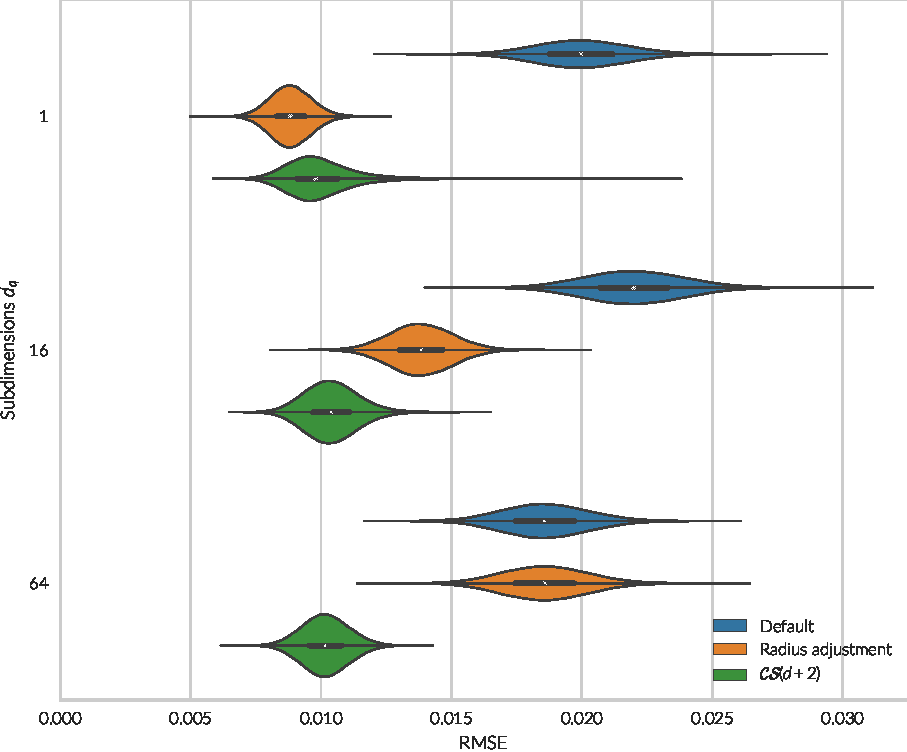
\includegraphics{figures/spaopt-repr}
    \caption[Distribution of the RMSE in the representation of unit-vectors]{Distribution of the RMSE in the representation of 64-dimensional unit-vectors. The violinplots visualize the distribution with a kernel-density estimate mirrored horizontally. The midline of shows a box plot with mean (white) and quartiles (thick black). Results obtained with the Nengo default parameters are blue, with the radius adjustment method from \textcite{gosmann216} are orange, and using the $\csdist(\dims + 2)$ distribution for intercepts and evaluation points are green. Along the y-axis the number of subdimensions $\dims_q$ represented in a single ensemble are arranged.}\label{fig:spaopt-repr}
\end{figure}

Besides pure representation it is common to compute dot products in the context of the SPA\@.
For the dot product the element-wise products are computed in separate product networks and summed afterwards.
In these product networks the sum (and difference) of the two input elements needs to be represented (see \cref{sec:product}) which means that the represented value is distributed according to the sum of two cosine similarity distributions in the general case.
However, the dot product is often used to check the similarity of two unit-vectors and a result of one should be obtained for identical vectors.
For identical vectors, the two inputs to the element-wise products will be the same and the sum will follow the distribution of a single input stretched out by a factor of 2.
Thus, it is appropriate to use the $\csdist(\dims + 2)$ distribution for intercepts and evaluation points in the product networks used for dot products.
In the general case of non-identical inputs, this might not be fully optimal, but still performs well (\cref{fig:spaopt-dot}).
It is also only minimally worse than the previous radius adjustment method.
\begin{figure}
    \centering
    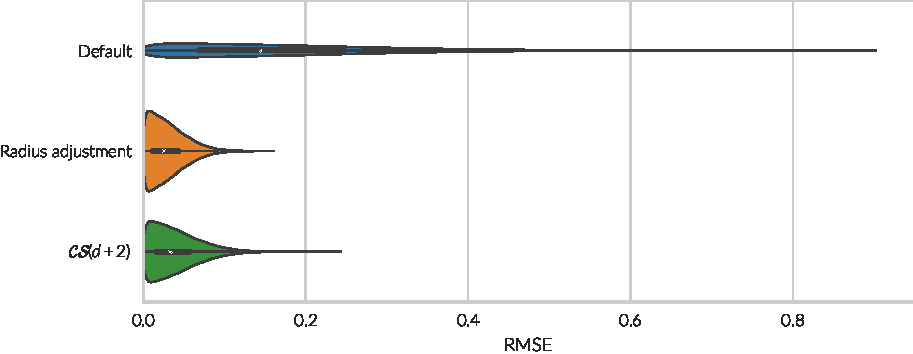
\includegraphics{figures/spaopt-dot}
    \caption[Distribution of the RMSE in dot product calculations]{Distribution of the RMSE in the calculation of dot products and vector lengths. The violinplots visualize the distribution with a kernel-density estimate. The midline of shows a box plot with mean (white) and quartiles (thick black).}\label{fig:spaopt-dot}
\end{figure}

%Finally, one might ask whether the cosine similarity distribution can also improve the calculation of circular convolutions.
%Unfortunately, the Fourier coefficients will have a different distribution.
%There is one important special case, with unitary vectors, where the absolute value of each coefficient is 1.
%Thus, the real and imaginary values will be distributed according to $\csdist(2)$ and the sum of two such random variables created in the product network (\cref{sec:product}) will then be distributed according to
%\begin{align}
    %p_{\csdist+\csdist}(z) &= \int_{z-1}^{z+1} \pcs(z; 2) \pcs(z - x; 2) \dif x \\
    %&= \uppi^2 \int_{z-1}^{z+1} \del{x^2 z^2 - x^2 - 2 x z^3 + 2 x z + z^4 - 2 z^2 + 1}^{-\frac{1}{2}} \dif x \text{.}
%\end{align}
%If vectors are known to be both unitary, this could allow for a more accurate neural calculation, but it is more common to have only one of the two vectors unitary.
%In the general case, no assumption about any vectors being unitary or non-unitary should be made and a uniform intercept distribution should be used with an appropriately scaled radius.

Furthermore, the benchmark was only run for 64 dimensions with \num{200} neurons per dimension.
But the same conclusions as in \textcite{gosmann216} can be expected to hold for different dimensionalities and neuron numbers.
Increasing the dimensionality will improve the benefit of adjusting the radius, or the intercept and evaluation point distributions.
Similarly, the neuron number can be reduced to achieve faster simulation times without an increase in error.
